\documentclass{article}

\usepackage{amsmath}
\usepackage[hidelinks]{hyperref}
\usepackage{amssymb}
\usepackage{tikz}
\usepackage{booktabs}

\begin{document}    
    \begin{table}[h]
        \centering
        \caption{Mapping Types}
        \begin{tabular}{lcccccc}
            \toprule
            & 1-to-1 & Onto & $\deg{a}$ & $\deg{b}$ & $|A|\ ?\ |B|$ & Fig. \\
            \midrule
            Not a function & & & & & & \ref{fig:not-a-func} \\
            Regular function & & & $= 1$ & & & \ref{fig:func} \\
            Injective & $\checkmark$ & & $= 1$ & $ \leq 1$ & $\leq$ & \ref{fig:injective} \\
            Surjective & & $\checkmark$ & $= 1$ & $\geq 1$ & $\geq$ & \ref{fig:surjective} \\
            Bijective & $\checkmark$ & $\checkmark$ & $= 1$ & $= 1$ & $=$ & \ref{fig:bijective} \\
            \bottomrule
        \end{tabular}
        
    \end{table}

    \begin{figure}[h]
        \centering
        \begin{tikzpicture}
            \node (a1) at (0, 0) {$1$};
            \node (a2) at (0, -1cm) {$2$};
            \node (a3) at (0, -2cm) {$0$};
            
            \node (b1) at (5cm, 0) {$2$};
            \node (b2) at (5cm, -1cm) {$1$};
            \node (b3) at (5cm, -2cm) {$0$};

            \draw[->] (a1) to (b1);
            \draw[->] (a2) to (b1);
            \draw[->] (a2) to (b2);
        \end{tikzpicture}
        \caption{Not a Function}
        \label{fig:not-a-func}
    \end{figure}
        
    \begin{figure}[h]
        \centering
        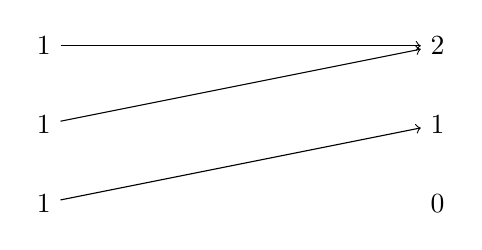
\begin{tikzpicture}
            \node (a1) at (0, 0) {$1$};
            \node (a2) at (0, -1cm) {$1$};
            \node (a3) at (0, -2cm) {$1$};
            
            \node (b1) at (5cm, 0) {$2$};
            \node (b2) at (5cm, -1cm) {$1$};
            \node (b3) at (5cm, -2cm) {$0$};

            \draw[->] (a1) to (b1);
            \draw[->] (a2) to (b1);
            \draw[->] (a3) to (b2);
        \end{tikzpicture}
        \caption{Function}
        \label{fig:func}
    \end{figure}

    \begin{figure}[h]
        \centering
        \begin{tikzpicture}
            \node (a1) at (0, 0) {$1$};
            \node (a2) at (0, -1cm) {$1$};
            \node (a3) at (0, -2cm) {$1$};
            
            \node (b1) at (5cm, 0) {$1$};
            \node (b2) at (5cm, -1cm) {$0$};
            \node (b3) at (5cm, -2cm) {$1$};
            \node (b4) at (5cm, -3cm) {$1$};

            \draw[->] (a1) to (b1);
            \draw[->] (a2) to (b3);
            \draw[->] (a3) to (b4);
        \end{tikzpicture}
        \caption{Injective Function}
        \label{fig:injective}
    \end{figure}

    \begin{figure}[h]
        \centering
        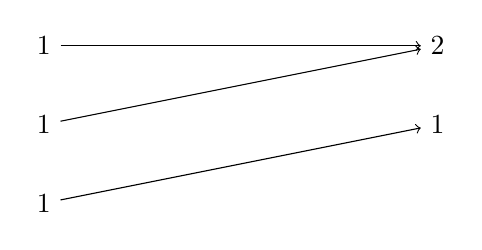
\begin{tikzpicture}
            \node (a1) at (0, 0) {$1$};
            \node (a2) at (0, -1cm) {$1$};
            \node (a3) at (0, -2cm) {$1$};
            
            \node (b1) at (5cm, 0) {$2$};
            \node (b2) at (5cm, -1cm) {$1$};

            \draw[->] (a1) to (b1);
            \draw[->] (a2) to (b1);
            \draw[->] (a3) to (b2);
        \end{tikzpicture}
        \caption{Surjective Function}
        \label{fig:surjective}
    \end{figure}

    \begin{figure}[h]
        \centering
        \begin{tikzpicture}
            \node (a1) at (0, 0) {$1$};
            \node (a2) at (0, -1cm) {$1$};
            \node (a3) at (0, -2cm) {$1$};
            
            \node (b1) at (5cm, 0) {$1$};
            \node (b2) at (5cm, -1cm) {$1$};
            \node (b3) at (5cm, -2cm) {$1$};

            \draw[->] (a1) to (b1);
            \draw[->] (a2) to (b2);
            \draw[->] (a3) to (b3);
        \end{tikzpicture}
        \caption{Bijective Function}
        \label{fig:bijective}
    \end{figure}
\end{document}
